\documentclass{bioinfo}


\copyrightyear{2005}
\pubyear{2005}
\bibliographystyle{bioinformatics}
\begin{document}
\firstpage{1}

\title[short Title]{Adding Some SPICE to DAS}
\author[Prli\'c \textit{et~al}]{Andreas Prli\'c \footnote{to whom correspondence should be addressed}, Thomas A. Down, Tim J. P. Hubbard\,}
\address{Wellcome Trust Sanger Institute
Wellcome Trust Genome Campus,
Hinxton, Cambridge, CB10 1SA, UK}
\maketitle

\begin{abstract}

The Distributed Annotation System (DAS) defines a communication protocol used 
to exchange biological annotations. It is motivated by the idea that annotations 
should not be provided by single centralized databases, but instead be spread 
over multiple sites. Data distribution, performed by DAS servers, is separated
from visualization, which is done by DAS clients. The original DAS protocol was 
designed to serve annotation of genomic sequences. We have extended the protocol 
to be applicable to macromolecular structures. Here we present SPICE, a new DAS
client that can be used to visualize protein sequence and structure annotations.

\section{Availability:}  \href{http://www.efamily.org.uk/software/dasclients/spice/}{http://www.efamily.org.uk/software/dasclients/spice/}

\section{Contact:} \href{ap3@sanger.ac.uk}{ap3@sanger.ac.uk}
\end{abstract}

\section{Introduction}

A variety of manual, computational, and experimental annotations of  biological data like genomes or proteins, are being developed by different groups all around the world. 
The DAS protocol allows data producers to share their results with the community without requiring 
aggregation into a central database (\cite{Dowell.Jokerst.ea:2001}). Resources 
like the EnsEMBL genome browser (\cite{ENSEMBL:2005}) use the DAS protocol to link new data to the 
browser and visualize it. Although originally designed to serve annotations of 
genomes, in the last year DAS has also received some interest from the protein-bioinformatics
community, largely because of the BioSapiens (\href{http://www.biosapiens.info/}{http://www.biosapiens.info/})
and eFamily (\href{http://www.efamily.org.uk/}{http://www.efamily.org.uk/}) projects.

DAS provides a simple convention how to encode e.g. a DNA or protein ``sequence'',
and its annotated ``features'' into simple XML documents that are exchanged via 
the Internet (\href{http://www.biodas.org/}{http://www.biodas.org/}). 
To make the DAS protocol applicable for protein structures we developed two 
extensions that allow alignments and 3D structure
information (\href{http://www.sanger.ac.uk/Users/ap3/DAS/}{http://www.sanger.ac.uk/Users/ap3/DAS/}) to be transmitted.
Using these extensions a variety of new DAS clients become possible.  For example,
pairwise or multiple alignments of chromosomes or protein sequences could be
visualized. Here we are using these extensions to support a new DAS client, SPICE,
that can be used to visualize annotations of protein sequences and protein
structures.

\section{The SPICE - DAS client}

SPICE is a Java program that can be started using Java Web Start by simply following a web
link. It accepts either a PDB (\cite{Berman.ea:2000}) or a UniProt code (\cite{uniprot:2004}) as an argument. If the application is started the first time, Web Start will download the 
program automatically. Once SPICE is running, it connects to the DAS 
registration service (\href{http://das.sanger.ac.uk/registry/}{http://das.sanger.ac.uk/registry/})
(to be published) to retrieve a list of available DAS servers. 

Four different types of DAS servers contribute to a complete SPICE display:
(1) A protein sequence server that provides the sequence. Typically this will be
a UniProt sequence, but because of the data independence achieved by using the
DAS protocol, it is  possible to use any other sequence source, if annotations
are provided using the other types of DAS servers.

(2) An alignment server that provides the alignment between the protein sequence
and its structure. At the time of submission of this manuscript the UniProt to
PDB alignment used in SPICE is based on the MSD mapping (\cite{EMSD:2003}).  If
other alignments are made available the user can choose between alternative
servers and compare the provided alignments.  The 3D structure of a
protein may have been resolved several times,  and a structure can consists of
several sequences. To deal with this many to many relationship, a window is
available that allows to choose which of the alignments to display. 

(3) A structure server, that serves the 3D coordinates displayed.  If a local 
PDB installation is available, SPICE can be configured to check there first when
looking for structure data.  If a required structure is not found, it is
automatically retrieved using the macromolecular structure DAS extension. 
 
(4) Several feature servers that provide pre-calculated annotations. These can
be served in either protein sequence position or PDB residue number coordinates. 
The registration server keeps track of which coordinate system is used by a
server to avoid confusion. At the time of submission of this manuscript the DAS
registration server contains 15 DAS servers provided by 7 different institutions
serving either UniProt or PDB annotations. The available annotations include 
active site definitions, domain assignments, and secondary structure
assignment. One of the DAS sources provided is a mapping of genomic features including
SNPs and intron/exon borders onto UniProt sequences. Using SPICE it is therefore
possible to visualize the location of DNA features on the protein structure.

\begin{figure}
\centerline{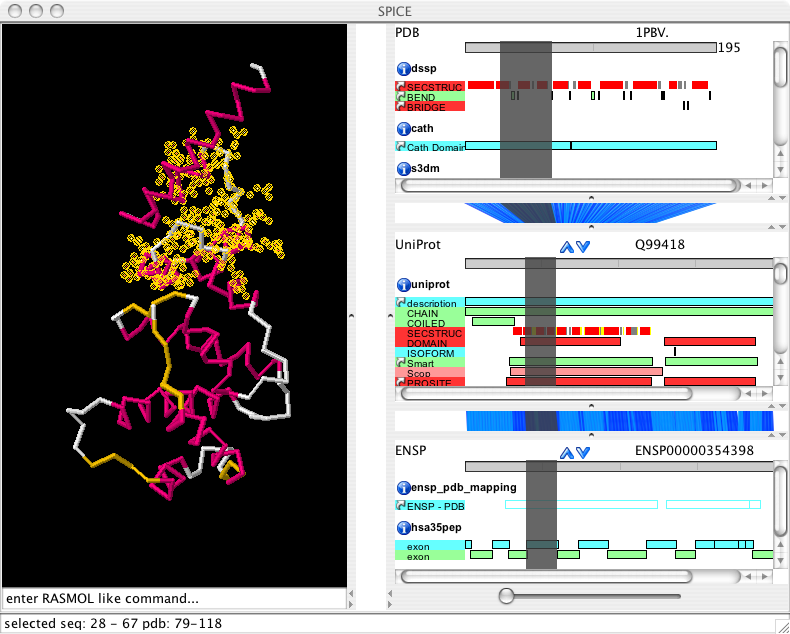
\includegraphics[width=250pt]{spice.png}}
\caption{The SPICE client allows users to browse through annotations of protein sequences and structures. It retreives data from different sites across the Internet via the DAS protocol.}\label{fig:01}
\end{figure}


The data retreived by SPICE is displayed in three main panels:
(1) The Structure panel provides a 3D visualization of the molecule using the
open source Jmol library (\href{http://www.jmol.org/}{http://www.jmol.org/}).
Jmol provides a powerful 3D visualization tool and can interpret 
RASMOL (\cite{rasmol:1995}) like scripting commands entered in a command line. 

(2)  Annotations provided by the distributed servers are displayed in a two
dimensional Feature panel, no matter if is provided in sequence positions or
PDB residue coordinates, since SPICE can project one onto the other. This is
required for the interaction between the sequence and structure panels. If an
annotation is selected, its location is shown in both the 3D structure and the
sequence panel.  The feature panel contains a listing of available annotations
making it easy to compare the annotations made by different methods. If the
user finds a particular source unreliable it is possible to disable it from the
display. 

(3) A Sequence panel that displays the amino acid sequence of the protein.  It
is possible to select regions and see the corresponding positions in the other
panels. The sequence can be searched  for motifs. 
 
It is possible to add new DAS sources to SPICE. The SPICE configuration allows 
access to local DAS sources that are still under development, or have not been 
registered with the DAS registration server. In this way SPICE can be used to 
evaluate new methods, by comparing new results
with the information that can be obtained from other resources. Since
features can contain links back to the original data, providing data with DAS
can also be used to advertise and draw attention to new methods.  Future
developments are to integrate SPICE  into the EnsEMBL web site. We will set up
DAS sources that provide alignments of UniProt sequences and PDB structures to
the EnsEMBL predicted peptides (ENSPs), through which it will be possible to
launch SPICE.  


\section{Conclusion}

SPICE is a tool to visualize protein sequence and protein structure annotations.
It utilizes the DAS protocol to retrieve its data from separate sites from the
Internet. It can be used to browse and compare the available annotations
for a particular protein as well as to compare the results of newly developed
methods with the pre-existing data.

\section{Availability}

The SPICE source code is available under the LGPL from 
\href{http://www.derkholm.net/svn/repos/spice/}{http://www.derkholm.net/svn/repos/spice/}.
Some modules are being made available through BioJava, which is also available
under LGPL from \href{http://www.biojava.org/}{http://www.biojava.org/}.


\section{Acknowledgments}

This work has been supported by the Medical Research Council.
Thanks to Rob Finn for suggesting the name SPICE and to Andreas K\"ah\"ari for
many feature suggestions. Thanks to everybody who is setting up DAS servers,
the system would not work without you!

\bibliography{references}

\end{document}




